\documentclass{resume} % Use the custom resume.cls style
\usepackage[left=0.4in,top=0.3in,right=0.4in,bottom=0.3in]{geometry} % Document margins
\usepackage{graphicx} % Required for including images
\newcommand{\tab}[1]{\hspace{.2667\textwidth}\rlap{#1}}
\newcommand{\itab}[1]{\hspace{0em}\rlap{#1}}
\graphicspath{ {../../images/} } % Relative location of the graphics files
\name{Jaman Uddin} % Your name
\address{+880 167 385-0025 \\ Uttara, Dhaka, Bangladesh}
\address{\href{mailto:zamaan.md19@gmail.com}{zamaan.md19@gmail.com} \\ \href{https://www.linkedin.com/in/rootprogrammer/}{linkedin.com/in/rootprogrammer} \\ \href{https://github.com/RootProgrammer}{github.com/RootProgrammer}}

\begin{document}

%----------------------------------------------------------------------------------------
%	PROFILE PICTURE
%----------------------------------------------------------------------------------------

\begin{figure}[t]
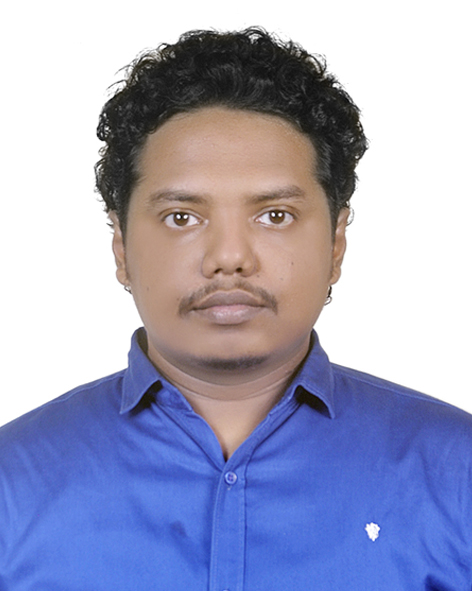
\includegraphics{jaman-01}
\centering
\end{figure}

%----------------------------------------------------------------------------------------
%	PROFESSIONAL SUMMARY
%----------------------------------------------------------------------------------------

\begin{rSection}{PROFESSIONAL SUMMARY}

{Dynamic Software Engineer with five years at imranslab, specializing in Python and Django with a strong focus on AI/ML integration. Proven leader in spearheading projects from inception to deployment, enhancing system efficiency and user engagement. Adept in Agile methodologies, committed to continual learning and development.}

\end{rSection}

%----------------------------------------------------------------------------------------
% SKILLS
%----------------------------------------------------------------------------------------
\begin{rSection}{SKILLS}

\renewcommand{\arraystretch}{1.5}
\begin{tabular}{@{} >{\bfseries}l @{\hspace{6ex}} >{\raggedright\arraybackslash}p{12cm}}
Software Development & Python, Flutter, Go, Django, TypeScript, JavaScript, ReactJS, Node.js\\
Technology Ecosystems & Django REST(DRF), FastAPI, RESTful API, Google Cloud Platform(GCP), RDBMS(Postgres, MySQL), NoSQL(MongoDB)\\
Quality Assurance \& DevOps & Selenium, Docker, Terraform, CircleCI\\
Development Tools & Git, GitHub, Jupyter Notebook, JIRA, Confluence\\
Collaboration Tools & Slack, Microsoft Teams, Windows, Debian, Ubuntu\\
\end{tabular}\\
\end{rSection}

%----------------------------------------------------------------------------------------
%	WORK HISTORY
%----------------------------------------------------------------------------------------

\begin{rSection}{WORK HISTORY}

\textbf{Software Engineer} \hfill Aug 2019 - Present\\
imranslab \hfill \textit{Montréal, QC (Remote)}
 \begin{itemize}
    \item Developed and launched a Job Finder platform, increasing user engagement by 30\% by integrating predictive AI algorithms, directly leading to a monthly active user increase.
    \item Enhanced the scalability of inventory management systems by 40\% by integrating real-time tracking features, resulting in improved logistical efficiency.
    \item Reduced operational costs by 20\% and improved deployment cycles by 30\% by transitioning legacy systems to a cloud-based infrastructure.
 \end{itemize}

\textbf{Software Development Intern} \hfill Feb 2019 - Jul 2019\\
imranslab \hfill \textit{Montréal, QC (Remote)}
 \begin{itemize}
    \item Successfully refactored 5000 lines of legacy Python code into a modular, maintainable structure adhering to SOLID principles, resulting in a 50\% improvement in code maintainability and a 30\% increase in development speed.
    \item Developed and implemented generative AI prompts for debugging complex system errors, enhancing troubleshooting efficiency by 25\% and reducing error resolution time by 40\%.
    \item Led the migration from local servers to cloud infrastructure, improving system scalability and reducing server downtime by 35\%, which enhanced overall system reliability by 45\%.
 \end{itemize}

\end{rSection} 

%----------------------------------------------------------------------------------------
%	PROJECTS
%----------------------------------------------------------------------------------------

\begin{rSection}{PROJECTS}

\begin{itemize}
    \item \textbf{AI-Enhanced Job Finder:} Engineered and optimized AI algorithms to refine resume evaluations, directly boosting match accuracy by 25\% and enhancing user satisfaction ratings by 30\%.
    \item \textbf{Trading Analysis Platform:} Re-architected a trading platform using Django, achieving a 35\% increase in processing efficiency and a 20\% reduction in latency.
    \item \textbf{Inventory Management System:} Spearheaded the design and implementation of a scalable inventory system that improved data accuracy by 50\% and reduced inventory costs by 15\%.
\end{itemize}

\end{rSection} 

%----------------------------------------------------------------------------------------
%	EDUCATION SECTION
%----------------------------------------------------------------------------------------

\begin{rSection}{EDUCATION}

{\bf B.Sc.(Engg.) in Computer Science and Engineering (CSE)}, Asian University of Bangladesh \hfill {2018 - 2022}

\end{rSection}

%----------------------------------------------------------------------------------------
% DISTINCTIONS
%----------------------------------------------------------------------------------------

\begin{rSection}{DISTINCTIVE MILESTONES \& PASSIONS} 

\begin{itemize} 
    \item \textbf{Achievements:} Participated in ICPC Regional 2019, Google Kick Start 2021; excelled in national coding contests.
    \item \textbf{Interests:} Passionate about emerging technologies, AI advancements, mentorship, and cinematic arts.
\end{itemize}

\end{rSection}

%----------------------------------------------------------------------------------------
%	LEADERSHIP
%----------------------------------------------------------------------------------------

\begin{rSection}{STRATEGIC COMMUNICATION \& LEADERSHIP EXCELLENCE} 

\begin{itemize}
    \item Masterfully utilized Confluence for end-to-end project documentation, boosting project transparency and improving team communication by 40\%, which significantly enhanced project delivery times and team cohesion.
    \item Cultivated a culture of innovation and collaboration, driving teams to exceed performance targets by up to 40\%, thereby increasing overall productivity and project success rates.
\end{itemize}

\end{rSection}

\end{document}
